\documentclass[../../main.tex]{subfiles}

\graphicspath{{../../image/}{../../figure/}}

\begin{document}

\subsection{神经 ODE 流}\label{subsection:ch18-神经ode流}

我们可以利用神经 ODE 来定义一个旨在构建易处理的标准化流模型的替代方法。神经 ODE 定义了一个从输入向量 $\bm{z}(0)$ 到输出向量 $\bm{z}(T)$ 的高度灵活的转换，其形式为如下微分方程：
\begin{align}
  \frac{\mathrm{d}\bm{z}(t)}{\mathrm{d}t}=\bm{f}\big(\bm{z}(t),\bm{w}\big).\label{align:ch18-流ode}
\end{align}
如果我们定义一个基于输入向量的基础分布 $p(\bm{z}(0))$，神经 ODE 就会随时间向前传播，从而得到每个 $t$ 值的分布 $p(\bm{z}(t))$，进而得到输出向量的分布 $p(\bm{z}(T))$。有研究 [Chen et al. (2018)] 指出，对于神经 ODE 来说，密度转换可以通过积分如下微分方程来计算（见\cref{exercise:ch18-08}）：

\begin{theorem}[连续流的瞬时变量替换]\label{theorem:ch18-瞬时变量替换}
设 $\bm{f}(\cdot,\bm{w})$ 在 $\mathbb{R}^{D}$ 上连续可微且导数有界，$\bm{z}(t)$ 是\eqref{align:ch18-流ode}以 $\bm{z}(0)$ 为初值的解，$p(\bm{z}(t),t)$ 表示 $\bm{z}(t)$ 的密度。若 $\bm{z}(0)$ 的密度为 $p_0$，则对 $\bm{z}(0)$ 的分布几乎处处的初值，
\begin{align}
  \frac{\mathrm{d}\ln p\big(\bm{z}(t)\big)}{\mathrm{d}t}=-\operatorname{tr}\left(\frac{\partial\bm{f}\big(\bm{z}(t),\bm{w}\big)}{\partial\bm{z}(t)}\right),\label{align:ch18-瞬时变量替换}
\end{align}
其中 $\partial\bm{f}/\partial\bm{z}(t)$ 表示 Jacobian 矩阵，其元素为 $\partial f_i/\partial z_j$。等价地，
\begin{align*}
  \ln p\big(\bm{z}(T)\big)=\ln p\big(\bm{z}(0)\big)-\int_{0}^{T}\operatorname{tr}\left(\frac{\partial\bm{f}\big(\bm{z}(t),\bm{w}\big)}{\partial\bm{z}(t)}\right)\mathrm{d}t .
\end{align*}
\end{theorem}

\begin{proof}（重构新增）
记 $\bm{\varphi}_t$ 为\eqref{align:ch18-流ode}的流映射（$\bm{z}(0)\mapsto\bm{z}(t)$），并记
\begin{align*}
  \bm{T}_t=\frac{\partial\bm{\varphi}_t}{\partial\bm{z}(0)},\qquad \bm{A}(t)=\frac{\partial\bm{f}}{\partial\bm{z}}\big(\bm{z}(t),\bm{w}\big).
\end{align*}
由 $\bm{z}(t)$ 对初值可微（$\bm{f}$ 的导数有界保证）及链式法则，$\bm{T}_t$ 满足线性矩阵微分方程
\begin{align*}
  \frac{\mathrm{d}\bm{T}_t}{\mathrm{d}t}=\bm{A}(t)\bm{T}_t,\qquad \bm{T}_0=\bm{I}.
\end{align*}

第一步，计算 $\det\bm{T}_t$。$\bm{T}_t$ 作为流映射的 Jacobian 恒可逆，故可用 Jacobi 公式 $(\det\bm{M})'=\det(\bm{M})\operatorname{tr}(\bm{M}^{-1}\bm{M}')$：
\begin{align*}
  \frac{\mathrm{d}}{\mathrm{d}t}\det\bm{T}_t=\det(\bm{T}_t)\operatorname{tr}\left(\bm{T}_t^{-1}\bm{A}(t)\bm{T}_t\right)=\det(\bm{T}_t)\operatorname{tr}\bm{A}(t),
\end{align*}
其中第二个等号用了迹的循环性。解这个一阶方程（初值 $\det\bm{T}_0=1$）得
\begin{align*}
  \det\bm{T}_t=\exp\left(\int_{0}^{t}\operatorname{tr}\bm{A}(s)\,\mathrm{d}s\right).
\end{align*}

第二步，用\cref{proposition:ch18-变量变换}把 $p_0$ 与 $p(\cdot,t)$ 联系起来。$\bm{\varphi}_t$ 是微分同胚，其逆的 Jacobian 是 $\bm{T}_t^{-1}$，故
\begin{align*}
  p\big(\bm{z}(t),t\big)=\frac{p_0\big(\bm{z}(0)\big)}{\left|\det\bm{T}_t\right|}.
\end{align*}
取对数并代入第一步的结果（$\det\bm{T}_t>0$）：
\begin{align*}
  \ln p\big(\bm{z}(t),t\big)=\ln p_0\big(\bm{z}(0)\big)-\int_{0}^{t}\operatorname{tr}\bm{A}(s)\,\mathrm{d}s .
\end{align*}
两端对 $t$ 求导（左端沿轨迹求全导数，$\ln p_0(\bm{z}(0))$ 与 $t$ 无关），即得\eqref{align:ch18-瞬时变量替换}。把\eqref{align:ch18-瞬时变量替换}从 $0$ 积分到 $T$ 即得定理中的累积形式。
\end{proof}

% SUPPLEMENT: parent=theorem:ch18-瞬时变量替换; kind=motivation; location=紧随其后的 remark（重构新增）
\begin{remark}（重构新增）
这条定理是连续流的核心，可以看成一维连续性方程 $\partial_t q+\partial_z(qf)=0$ 的积分形式，也可以看成离散流\eqref{align:ch18-change-var}的“无穷小版本”：在极短时间 $\delta t$ 内，流映射近似为 $\bm{z}+\delta t\,\bm{f}(\bm{z})$，其 Jacobian 是 $\bm{I}+\delta t\,\bm{A}$，由 $\det(\bm{I}+\delta t\bm{A})=1+\delta t\operatorname{tr}\bm{A}+\mathcal{O}(\delta t^{2})$ 得
\begin{align*}
  \ln p\big(\bm{z}(t+\delta t)\big)-\ln p\big(\bm{z}(t)\big)\approx-\delta t\operatorname{tr}\bm{A}(t),
\end{align*}
除以 $\delta t$ 并取极限就是\eqref{align:ch18-瞬时变量替换}。\cref{exercise:ch18-08}在一维情形用“体积（长度）守恒”给出了这个推导。

条件方面：$\bm{f}$ 连续可微且导数有界，保证流映射是微分同胚、$\bm{T}_t$ 恒可逆，从而 Jacobi 公式可用；若只假设 $\bm{f}$ Lipschitz，解仍存在唯一，但 $\bm{T}_t$ 的存在需要 $\bm{f}$ 可微。定理的结论是“几乎处处”的，因为\cref{proposition:ch18-变量变换}中的密度只在几乎处处意义下确定。定理中的累积形式还需要 $\operatorname{tr}\bm{A}(t)$ 在 $[0,T]$ 上可积，这在导数有界时自动成立。

符号的含义：$\operatorname{tr}\bm{A}>0$ 表示流在局部膨胀体积，密度随之下降（负号）；$\operatorname{tr}\bm{A}<0$ 表示压缩，密度上升。这与\cref{figure:ch18-连续流}中“流线分开处密度降低、靠拢处密度增加”的图像一致。
\end{remark}

这个积分操作可以使用标准 ODE 求解器来完成。同样，可以通过从基础分布 $p(\bm{z}(0))$ 中采样来获得这个密度的样本，这个基础分布可以是一个简单的分布，如 Gauss 分布，并支持使用 ODE 求解器再次整合［\eqref{align:ch18-流ode}］，以便将值传播到输出。

\begin{definition}[连续标准化流]\label{definition:ch18-连续标准化流}
设 $p(\bm{z}(0))$ 是输入向量上的基础分布，$\bm{z}(t)$ 满足\eqref{align:ch18-流ode}，$p(\bm{z}(t))$ 按\eqref{align:ch18-瞬时变量替换}演化。称由\eqref{align:ch18-流ode}定义的、把 $p(\bm{z}(0))$ 变换为 $p(\bm{z}(T))$ 的标准化流为\textbf{连续标准化流}（continuous normalizing flow），并把定理中的累积形式称为它的密度计算公式。
\end{definition}

% SUPPLEMENT: parent=definition:ch18-连续标准化流; kind=motivation; location=紧随其后的 remark（重构新增）
\begin{remark}（重构新增）
连续标准化流把\cref{definition:ch18-标准化流}中的“有限个可逆层”换成了“一个连续时间的过程”：层数不再是整数，而是由求解器自适应选择的求值点；每层的对数行列式贡献被换成 $\operatorname{tr}\bm{A}(t)$ 在时间上的积分。因此它是离散标准化流的“无穷深”极限，也是\cref{proposition:ch18-分层流}中“各层对数行列式之和”的连续版本——求和变成了积分。

条件方面：基础分布要简单、可采样、对数密度可算（例如标准 Gauss）；$\bm{f}$ 要满足\cref{theorem:ch18-瞬时变量替换}的正则性条件，使流映射是微分同胚，从而\eqref{align:ch18-流ode}确实定义了一个可逆变换。与离散流不同的是，这里不需要显式构造逆映射：反向只需把时间从 $T$ 积分回 $0$，同一个求解器即可完成。

一个实用上的差别：离散流的层数固定，计算图固定，反传直接可用；连续流的“层”由求解器决定，其反向需要伴随方法（见\cref{subsection:ch18-ode-backprop}），这正是下一段要说明的。
\end{remark}

连续标准化流可以使用适用于神经 ODE 的伴随灵敏度方法进行训练，该方法可以看作反向传播的连续时间等价物（参见\cref{subsection:ch18-ode-backprop}）。

\begin{figure}[htbp]
  \centering
  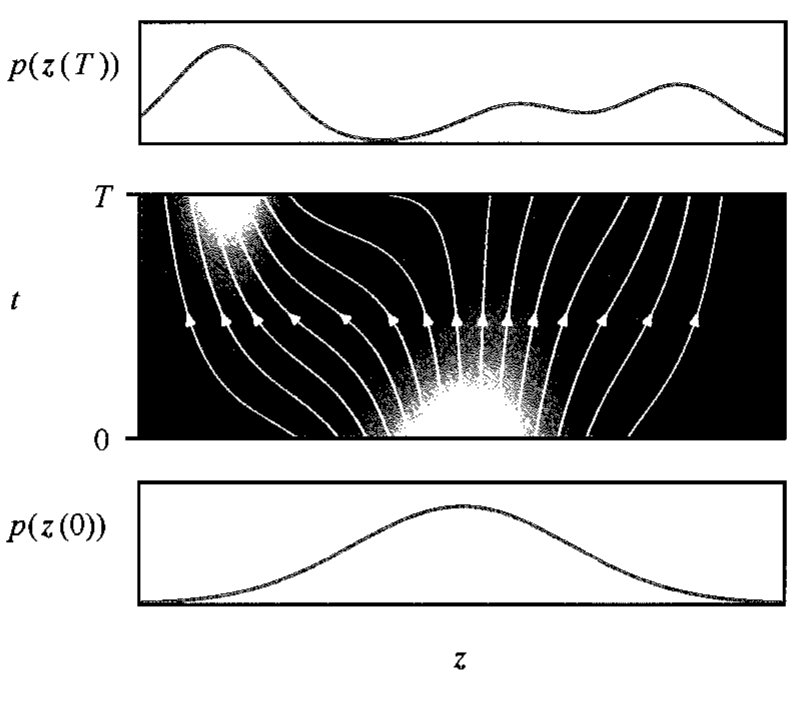
\includegraphics[width=0.62\textwidth]{ch18-fig505-cnf.png}
  \caption{连续标准化流的示意图，这里展示了 $t=0$ 时刻的一个简单 Gauss 分布是如何通过连续转换变成 $t=T$ 时刻的一个多峰分布的。当流线分开时，密度降低；当流线靠拢时，密度增加}
  \label{figure:ch18-连续流}
\end{figure}

由于\eqref{align:ch18-瞬时变量替换}涉及 Jacobian 矩阵的\textbf{迹}而不是行列式（行列式出现在离散标准化流中），它可能看起来更具计算效率。

\begin{proposition}[密度计算的代价]\label{proposition:ch18-密度代价}
设 $D$ 为数据维数，$\bm{A}$ 为 $D\times D$ 矩阵。则：（i）计算 $\det\bm{A}$ 一般需要 $\mathcal{O}(D^{3})$ 次运算，而计算 $\operatorname{tr}(\bm{A})$ 只需 $\mathcal{O}(D)$ 次运算；（ii）若 $\bm{A}$ 是三角矩阵，则 $\det\bm{A}$ 是对角元之积，也只需 $\mathcal{O}(D)$ 次运算；（iii）形成 $\bm{A}=\partial\bm{f}/\partial\bm{z}$ 需要 $D$ 次 Jacobian-向量积，每次的代价与前向求值 $\bm{f}$ 同阶（记为 $\mathcal{O}(D)$），故精确计算 $\operatorname{tr}(\bm{A})$ 或三角矩阵的行列式共需 $\mathcal{O}(D^{2})$ 的成本；（iv）若改用\eqref{align:ch18-迹估计}的随机估计，只需 $M$ 次矩阵-向量积，代价为 $\mathcal{O}(MD)$，取 $M=1$ 时为 $\mathcal{O}(D)$。
\end{proposition}

\begin{proof}（重构新增）
（i）一般矩阵的行列式用 LU 分解计算，分解本身是 $\mathcal{O}(D^{3})$，再乘对角元是 $\mathcal{O}(D)$；迹只是把 $D$ 个对角元相加，是 $\mathcal{O}(D)$。

（ii）三角矩阵的 LU 分解不需要消元（行列式即对角元之积），故为 $\mathcal{O}(D)$。

（iii）$\bm{A}$ 的第 $j$ 列是 $\partial\bm{f}/\partial z_j$，可用一次 Jacobian-向量积（或反向的向量-Jacobian 积）得到，其代价与一次前向求值 $\bm{f}$ 同阶；对 $D$ 个方向各做一次即为 $\mathcal{O}(D^{2})$。得到全部对角元后求和是 $\mathcal{O}(D)$，被 $\mathcal{O}(D^{2})$ 吸收。

（iv）\eqref{align:ch18-迹估计}只需对每个样本计算 $\bm{\varepsilon}_m^{\mathsf T}\bm{A}\bm{\varepsilon}_m$，即一次向量-Jacobian 积再与 $\bm{\varepsilon}_m$ 内积，代价 $\mathcal{O}(D)$；$M$ 个样本共 $\mathcal{O}(MD)$。
\end{proof}

% SUPPLEMENT: parent=proposition:ch18-密度代价; kind=motivation; location=紧随其后的 remark（重构新增）
\begin{remark}（重构新增）
这条结论解释了连续流相对于离散流的计算优势与代价。优势是：离散流要对每层算一次行列式，即便每层是三角的也要 $\mathcal{O}(D)$，层数一多就累积；连续流把“每层的行列式”换成“迹的时间积分”，而迹的精确计算只需 $\mathcal{O}(D^{2})$（主要开销是形成 Jacobian），与层数无关。代价是：迹仍然需要 $D$ 次 Jacobian-向量积，当 $D$ 很大时 $\mathcal{O}(D^{2})$ 仍不可忽视，于是有了下面的随机估计。

条件方面：（i）中的 $\mathcal{O}(D^{3})$ 是一般稠密矩阵的代价，若 $\bm{A}$ 有特殊结构（三角、低秩、对角加低秩）则可大幅降低；（iii）中“每次 Jacobian-向量积与前向同阶”对逐层网络成立，对一般黑箱向量场则以实际求值代价为准。原文把“计算 Jacobian 的各个元素需要单独的前向传播”计为 $\mathcal{O}(D)$ 次运算，与这里的记账一致：$D$ 次求值，每次 $\mathcal{O}(D)$。
\end{remark}

然而，通过使用 Hutchinson 的迹估计器（Grathwohl et al., 2018），我们可以将计算迹的成本降低到 $\mathcal{O}(D)$。对于矩阵 $\bm{A}$，迹的形式为
\begin{align}
  \operatorname{tr}(\bm{A})=\mathbb{E}_{\bm{\varepsilon}}\left[\bm{\varepsilon}^{\mathsf T}\bm{A}\bm{\varepsilon}\right],\label{align:ch18-hutchinson}
\end{align}
其中 $\bm{\varepsilon}$ 是一个零均值、单位协方差的随机向量，例如 Gauss 分布 $\mathcal{N}(\bm{0},\bm{I})$。对于一个特定的 $\bm{\varepsilon}$，矩阵-向量乘积 $\bm{A}\bm{\varepsilon}$ 可以使用反向的自动微分在单次传递中高效计算。然后我们可以使用有限数量的样本来近似矩阵的迹，形式如下：
\begin{align}
  \operatorname{tr}(\bm{A})\approx\frac{1}{M}\sum_{m=1}^{M}\bm{\varepsilon}_m^{\mathsf T}\bm{A}\bm{\varepsilon}_m .\label{align:ch18-迹估计}
\end{align}

\begin{proposition}[迹估计量的无偏性]\label{proposition:ch18-迹估计无偏}
设 $\bm{\varepsilon}$ 是零均值、协方差为 $\bm{I}$ 的 $D$ 维随机向量，$\bm{A}$ 为 $D\times D$ 实矩阵。则
\begin{align*}
  \mathbb{E}\left[\bm{\varepsilon}^{\mathsf T}\bm{A}\bm{\varepsilon}\right]=\operatorname{tr}(\bm{A}).
\end{align*}
因此对任意 $M\geqslant1$ 与独立同分布的 $\bm{\varepsilon}_1,\cdots,\bm{\varepsilon}_M$，\eqref{align:ch18-迹估计}右端的期望恰为 $\operatorname{tr}(\bm{A})$，即该估计量是无偏的。
\end{proposition}

\begin{proof}（重构新增）
由二次型的展开，
\begin{align*}
  \mathbb{E}\left[\bm{\varepsilon}^{\mathsf T}\bm{A}\bm{\varepsilon}\right]=\mathbb{E}\left[\sum_{i,j}A_{ij}\varepsilon_i\varepsilon_j\right]=\sum_{i,j}A_{ij}\,\mathbb{E}\left[\varepsilon_i\varepsilon_j\right].
\end{align*}
$\bm{\varepsilon}$ 零均值、协方差为 $\bm{I}$，即 $\mathbb{E}[\varepsilon_i]=0$、$\mathbb{E}[\varepsilon_i\varepsilon_j]=\delta_{ij}$，故上式等于 $\sum_{i}A_{ii}=\operatorname{tr}(\bm{A})$。

对 $M$ 个独立样本，由期望的线性性，
\begin{align*}
  \mathbb{E}\left[\frac{1}{M}\sum_{m=1}^{M}\bm{\varepsilon}_m^{\mathsf T}\bm{A}\bm{\varepsilon}_m\right]=\frac{1}{M}\sum_{m=1}^{M}\mathbb{E}\left[\bm{\varepsilon}_m^{\mathsf T}\bm{A}\bm{\varepsilon}_m\right]=\operatorname{tr}(\bm{A}),
\end{align*}
与 $M$ 无关，故估计量无偏。
\end{proof}

% SUPPLEMENT: parent=proposition:ch18-迹估计无偏; kind=motivation; location=紧随其后的 remark（重构新增）
\begin{remark}（重构新增）
无偏性只用到前两阶矩，与 $\bm{\varepsilon}$ 的具体分布无关；取 Gauss 只是为了让采样方便、并便于分析方差。这里不需要 $\bm{A}$ 对称，也不需要它正定——二次型的期望只依赖对角元，非对角元在 $\mathbb{E}[\varepsilon_i\varepsilon_j]=\delta_{ij}$ 处被消掉。

\textbf{关于“单位协方差”。} 原文举例写作 $\mathcal{N}(0,1)$，而在 $D$ 维情形应理解为每个分量独立的标准 Gauss 分布，即 $\bm{\varepsilon}\sim\mathcal{N}(\bm{0},\bm{I})$；若各分量方差不等于 $1$，则 $\mathbb{E}[\bm{\varepsilon}^{\mathsf T}\bm{A}\bm{\varepsilon}]=\operatorname{tr}(\bm{A}\bm{\Sigma})$，不再是 $\operatorname{tr}(\bm{A})$，这会引入系统偏差。

方差方面：$\operatorname{Var}(\bm{\varepsilon}^{\mathsf T}\bm{A}\bm{\varepsilon})$ 与 $\|\bm{A}\|_F^{2}$ 同阶，因此 $M$ 个样本把标准差降到 $1/\sqrt{M}$ 量级。$M=1$ 时估计有噪声，但它是无偏的，且噪声会与随机梯度下降的其它噪声一起被平均掉，这正是下一段所说的“不太重要”。
\end{remark}

实践中，我们可以设置 $M=1$ 并只使用一个样本对每个新的数据点进行刷新。虽然这是一个有噪声的估计，但由于它是噪声随机梯度下降过程的一部分，这可能显得不太重要。重要的是，它是无偏的，这意味着估计器的期望等于真实值（参见\cref{exercise:ch18-11}）。

通过使用一种名为流匹配（flow matching）的技术（参见\cref{chapter:ch20-扩散模型}），可以显著提高连续标准化流的训练效率（Lipman et al., 2022）。这使得标准化流更接近于扩散模型，避免了在积分器中进行反向传播，同时大幅减少内存需求，实现了更快的推理和更稳定的训练。

\end{document}
